\chapter{Methodology}
\label{chap:Methodology}

This chapter is about describing the methodology and developments to achieve the project goals. 
Firstly, by elaborating on the workings of classification process in the processing thread. Moving on, delving into the operational sequences of the controller thread. Lastly, providing an explanation on the implementation of the controller.


\section{Classification}
\label{sec:section_classification}

The classification is a key step in this routine and for being able to be used in multipurpose applications the classification must be able to run in real-time, which means it must be fast and automatic.
The goal is to improve and apply approaches of non-visual spraying classification using the current data collected from the system.

\subsection{Statistical Analysis}
In Sjaaks\cite{Sjaaks} work, the author exposed signal characteristics that can be used to classify the actual spraying mode with a sample of measured current using both time and frequency domain analysis.
It is acquired the current data frame of 0.5s with 100 kHz as sampling frequency, with each current sample as 50 thousand current values. Through statistical analysis in these values such as mean, median and standard deviation the classification is done. 
Figure \ref{fig:sjaaks_statistical_class} illustrate data samples being classified using Sjaaks\cite{Sjaaks} method.

\begin{figure}[H]
    \centering
    \resizebox{80mm}{!}{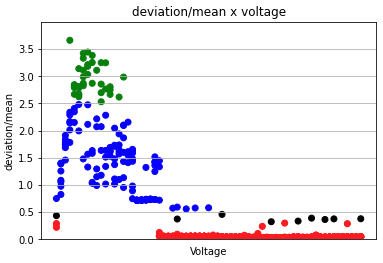
\includegraphics{Figuras/report2/data3_sjaaksgraph2.png}}
    \caption{Sample classification using statistical values. Colors: Green = Dripping; Blue = Intermittent; Red = Cone Jet.}
    \label{fig:sjaaks_statistical_class}
\end{figure}

 

This classification by statistical analysis was already implemented in the software library made by the previous student \cite{Monica}.
This method was capable of only classifying dripping, intermittent and cone jet modes. Also in her work, Monica extended the classification to corona or discharge detection.
My contribution was to integrate her work on my control loop model and extend the classification for the multi jet.

To classify the multi jet, after running many steps experiments it was noticed that the multi jet signal has a similar shape as the cone jet but with a step in its current mean, also the cone jet current was almost fixed in all its voltage range. 
These effects were exposed by Ryan\cite{Ryan}. In his work he defines the relation between current per jet in both cone jet and multi jet modes.

With that, it was implemented the classification of the multi jet when the current mean is 1.14 above the expected cone jet current mean. 
The cone jet current can be calculated by the scaling laws \ref{sec:scalling-laws} formula.
The factor value of 1.14 was found by repeating a lot of experiments with the same liquid (pure ethanol), but varying the flow rate and the voltage. This factor value is just applied for pure ethanol, the liquid used in all experiments in this work.
The classification in the algorithm was divided in three steps as shown below.

        - Sjaak Classification -> Classifies Dripping, Intermittent and Cone Jet
        
        - Monica Classification -> Classifies Corona Sparks

        - João Classification -> Classifies Multi Jet

	The algorithm \ref{alg:statistical_class} shows the implemented classification and works in the following way:

	\begin{algorithm}
        \caption{Statistical Classification}\label{alg:statistical_class}
        \begin{algorithmic}
        \Function{statistical\_classification}{$sample$} 

            \State $spray\_mode \gets "Undefined"$;
            \State $mean \gets sample.mean$; 
            \State $std\_deviation \gets sample.std\_deviation$;
            \State $median \gets sample.median$;
            
            \If{ $mean / std\_deviation$ > 2.5}
                \Comment{Sjaak classification \cite{Sjaaks}} 
                \State $spray\_mode \gets "Dripping"$;
            \ElsIf{$ 2.5 < mean / std\_deviation < 2.5 \And mean / std\_deviation > 0.3 $}
                \State $spray\_ mode \gets "Intermittent"$;
            \ElsIf{ $mean / std\_deviation$ < 0.3}
                \State $spray\_ mode \gets "Cone Jet"$;
                \State $cone\_jet\_mean \gets mean$;
            \EndIf

            \If{ $mean / std\_deviation$ > 2.5}
                \Comment{Monica classification \cite{Monica}} 
            \EndIf

            \If{ $spray\_mode == "Cone Jet"$}
                \Comment{João classification} 
                \If{ $cone\_jet\_mean > 1.14 \times mean$}
                    \State $spray\_ mode \gets "Multi Jet"$;
                \EndIf
            \EndIf

            \Return $spray\_ mode$;
        \EndFunction
        \end{algorithmic}
    \end{algorithm}



\section{Routine Sequences}
\label{sec:routine_sequences}

    The program developed is capable of running different types of routines and with an easy way to implement new strategies.
    Continuing the methodology, in the setup json file there is a "sequence" attribute which can be chosen between "ramp", "step", "map" or "control".
    The controller thread will manage what the algorithm must do for each sequence.
    Following the control model in Figure\ref{fig:control_model_fig}, the controller outputs (voltage and flow rate) are the actuators signal.
    The sampling rate is fixed to 0.5 seconds for all the experiments, and it's managed by the data\_acquisiton\_thread\ref{subsec:data_aquisition}.


\subsection{Ramp}

The ramp sequence is simply done by sending one command to the power supply to perform a ramp in the voltage with initial, final and slope values.
The flow rate for this sequence is constant, and the experiment consists in a voltage range scan.

\subsection{Step}
\label{subsec:step_routine}

The step sequence is done by the same command send to the power supply but with the maximum slope value in order to proximate of a step signal.
By waiting a certain defined \emph{step\_time} and repeating the command in a loop until it gets into the final voltage, as represented in algorithm \ref{alg:stepping_algorithm}.


\begin{algorithm}
    \caption{STEP sequence in controller thread}\label{alg:stepping_algorithm}
    \begin{algorithmic}
    \Procedure{STEP}{$voltage\_start,voltage\_stop$} 
        \State $voltage \gets voltage\_start$
        \While{$voltage \leq voltage\_stop$} \Comment{scanning voltage range}
            \State \Call{send\_voltage\_command}{voltage}
            \State \Call{sleep}{step \_time}
            \State $voltage \gets voltage + step\_size$
        \EndWhile
    \EndProcedure

    \end{algorithmic}
\end{algorithm}

\subsection{Map}

The map that will be explained below is the most relevant sequence in this work. This type of experiment saves human work and time, create a precise analysis and can be compared with previous works for validation of methodology.
The purpose is to map the operational window, seen in Figure \ref{fig:map3Data_fig}, that can be defined where the cone jet spraying mode can be stabilized based on the flow rate, voltage and the setup configuration.

The map was inspired in Gañan-Calvo\cite{gananCalvo} work where he points how liquid conductivity influences the cone jet stability island. 

\begin{figure}[H]
    \center
    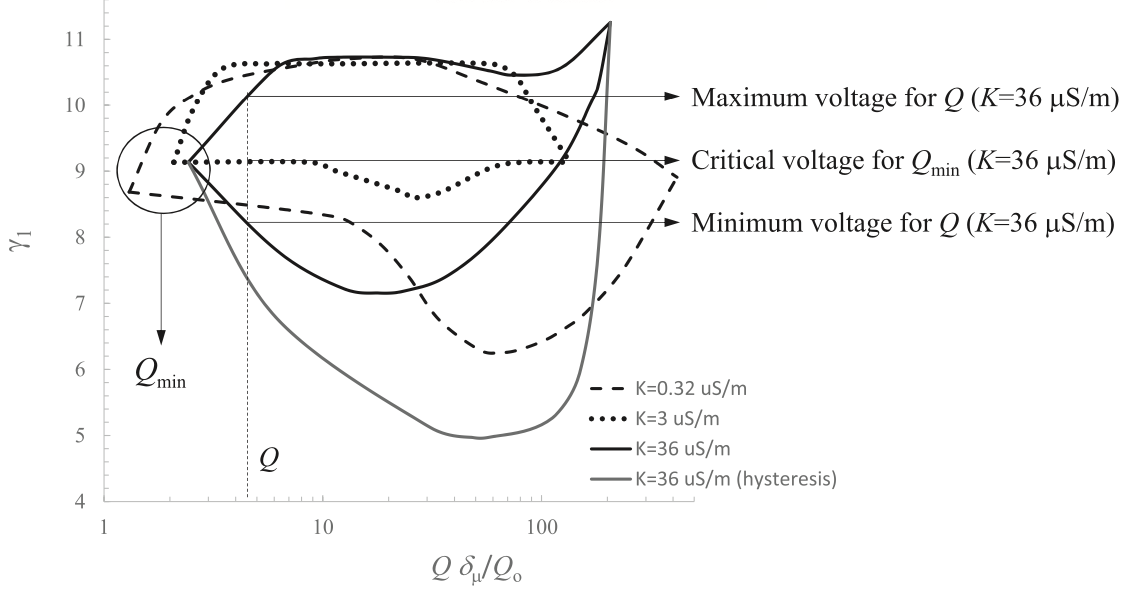
\includegraphics[width=13cm]{Figuras/ganan_calvo_map.png}
    \caption{Domains of existence (stability) of Taylor Cone Jets. \cite{gananCalvo} . The window formed by these points is where the system operated in the stable cone-jet. Operational windows depend on the liquid and configuration setup. Different windows are represented for different liquid conductivity. The X and Y axis are non-dimensional representation of electric potential and liquid flow rate, respectively.}
    \label{fig:ganan_calvo_fig}
\end{figure}

To reach certain map it is necessary to traverse flow rate and voltage values acquiring samples.
The flow rate (X axis) and voltage (Y axis) values for each experiment can be configured in the setup.json file.
The algorithm for this sequence is a loop of the step sequence\ref{subsec:step_routine} for each flow rate chosen, and it is represented in the algorithm \ref{alg:mapping_algorithm}.


    \begin{algorithm}
        \caption{MAP sequence in controller thread}\label{alg:mapping_algorithm}
        \begin{algorithmic}
        \Procedure{MAP}{$flowrate\_values$} 
            \ForAll{flowrate\_values}  \Comment{scanning in the flowrate range}
                \State \Call{send\_flowrate\_command}{flowrate}
                \State $voltage \gets voltage\_start$
                \While{$voltage \leq voltage\_stop$} \Comment{scanning in the voltage range}
                    \State \Call{send\_voltage\_command}{voltage}
                    \State \Call{sleep}{step \_time}
                    \State $voltage \gets voltage + step\_size$
                \EndWhile
            \EndFor
        \EndProcedure

        \end{algorithmic}
    \end{algorithm}

    In Figure \ref{fig:map2Data_fig} it can be seen the data acquired in this mapping experiments. The liquid used is pure ethanol. 
    Note that the experiment is composed of loops that increase voltage, change flow rate and repeat.

    \begin{figure}[H]
        \center
        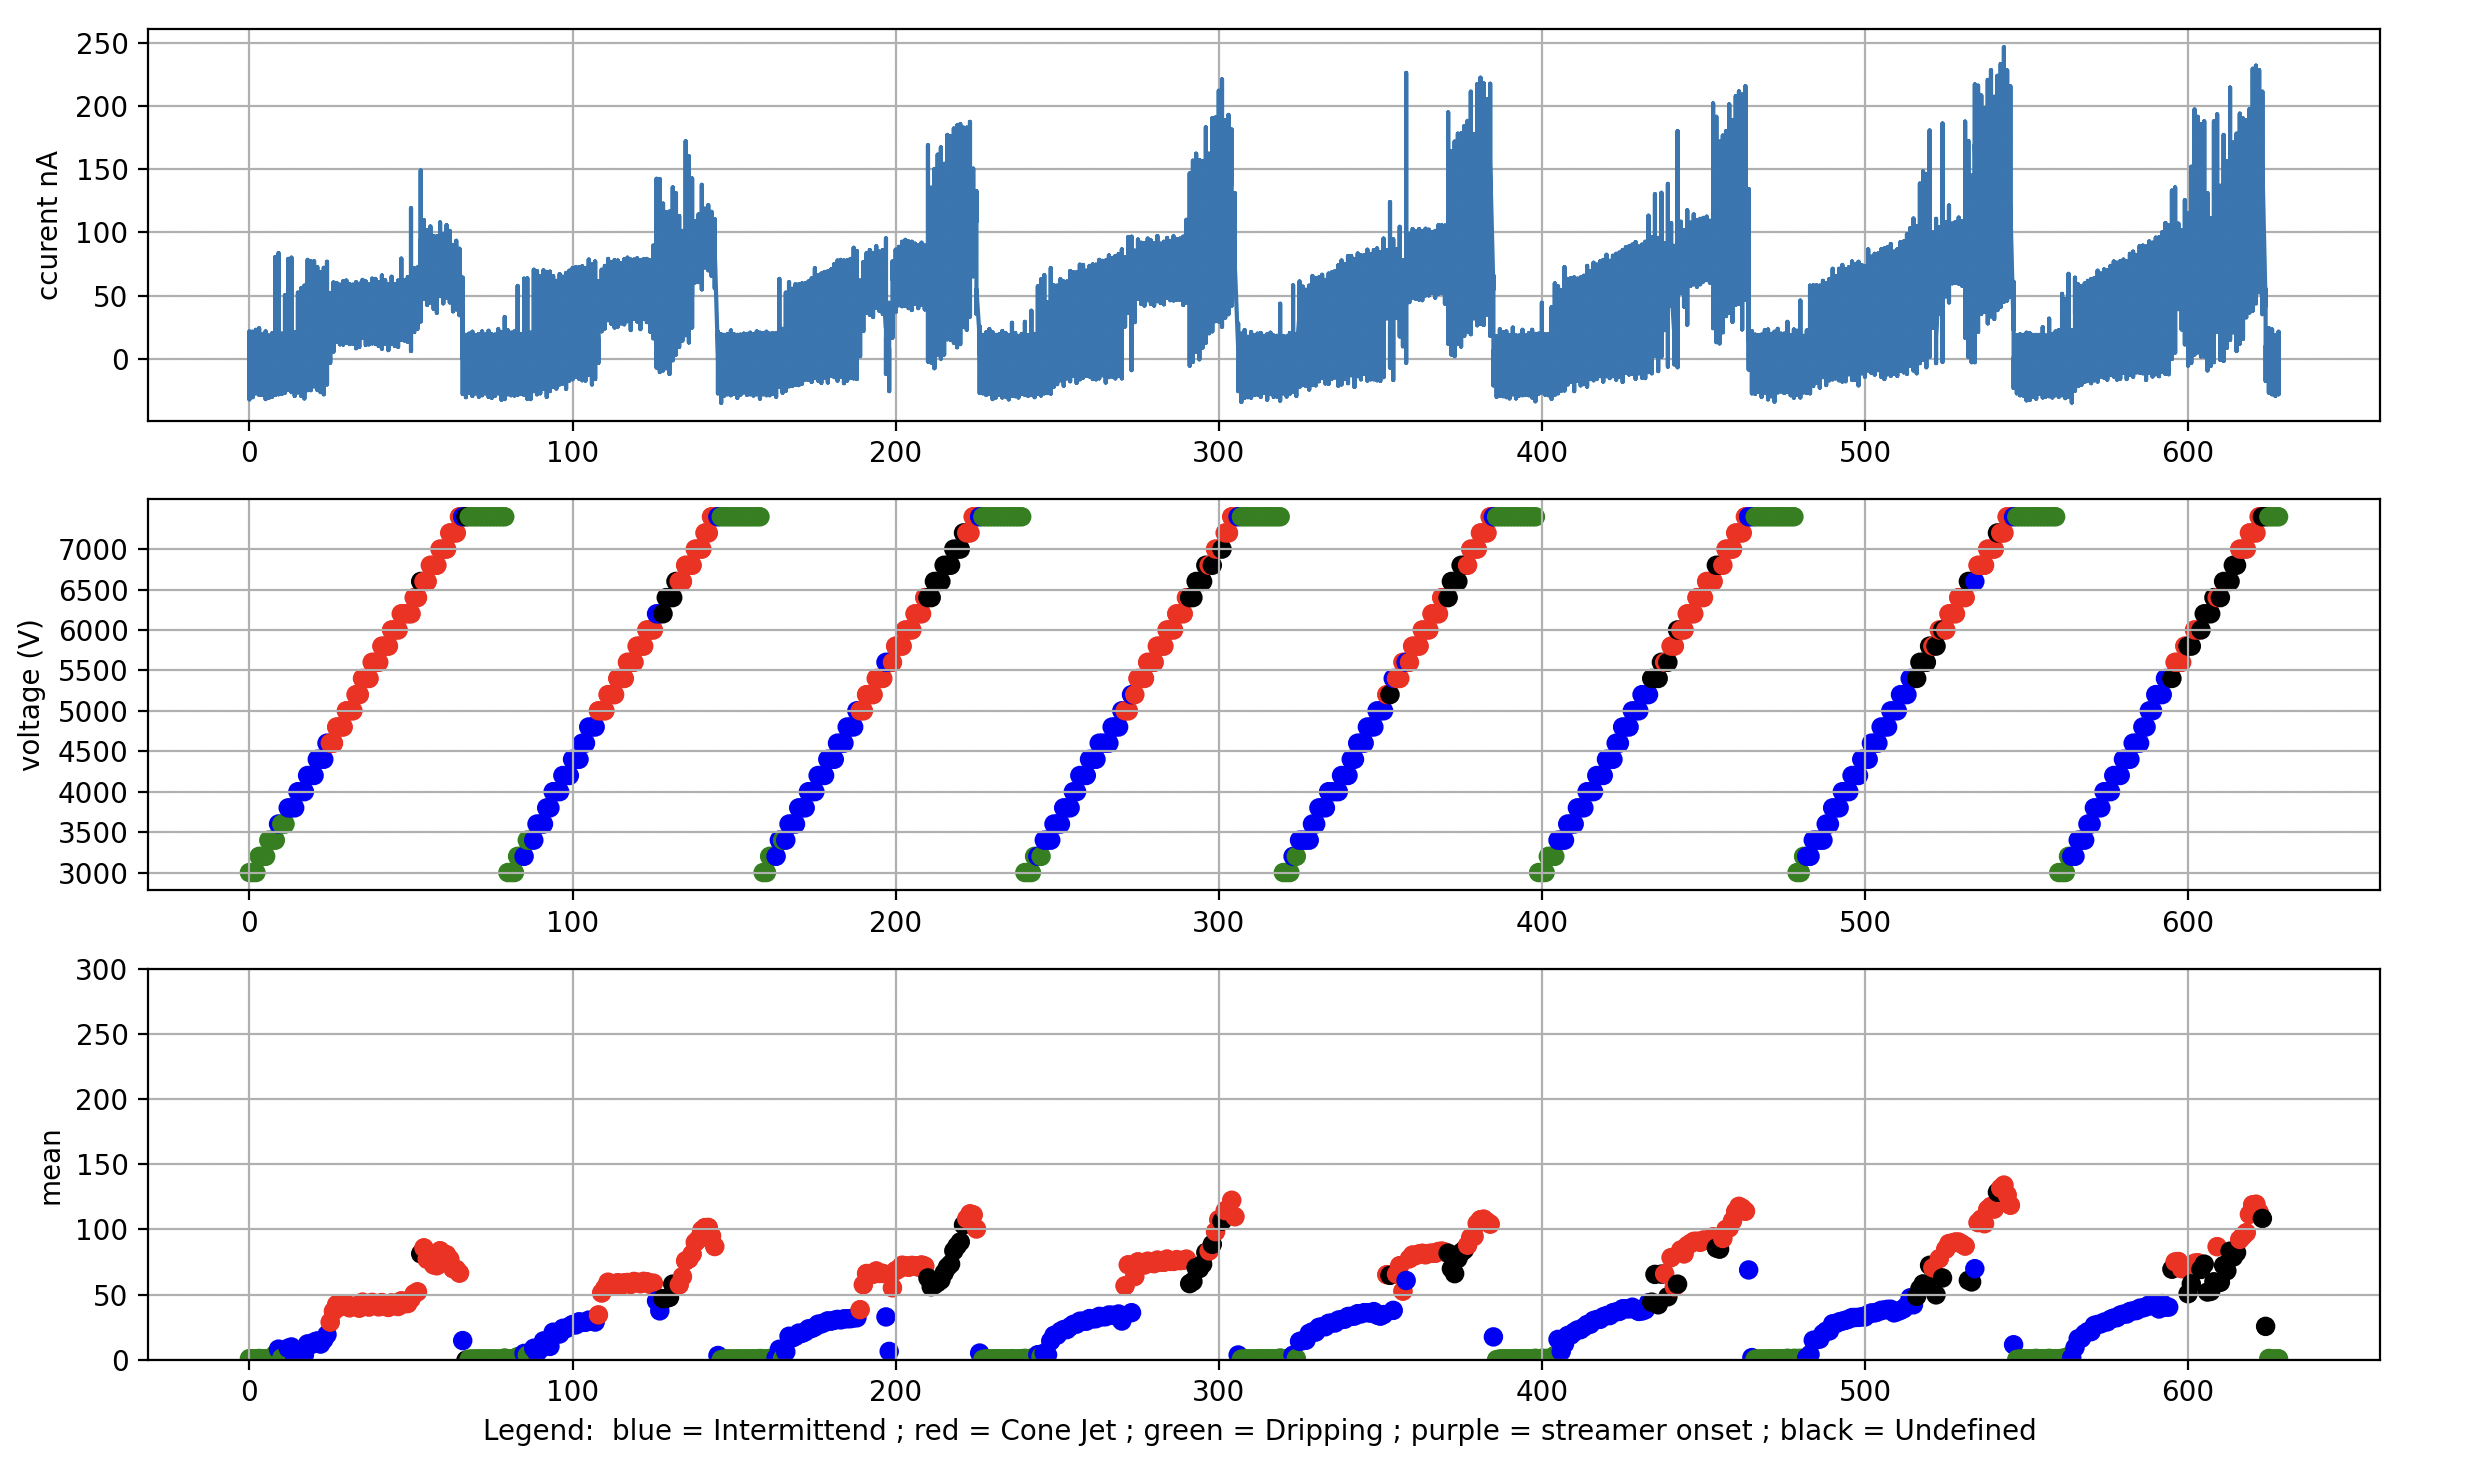
\includegraphics[width=15cm]{Figuras/report2/map2Data.png}
        \caption{Mapping Experiment data collected. The Figure has 3 graphs with shared x-axis representing the samples collected. The first is the current values collected through all the experiment.
        The second is the voltage values applied in each window of data collected. The colors represent the spraying classification defined in the routine.
        The third graph shows the current mean value of each data sample.}
        \label{fig:map2Data_fig}
    \end{figure}

    With all the data collected, classified and saved in real time, further analysis and studies can be done. For example, Figure \ref{fig:map3Data_fig} illustrate the data automatically classified and displayed in a Voltage X Flow rate range of spraying modes with a specific liquid setup so that a comparison on automatic results with previous researches can be done, such as showed in Figure \ref{fig:ganan_calvo_fig}, validating the algorithm.

    \begin{figure}[H]
        \center
        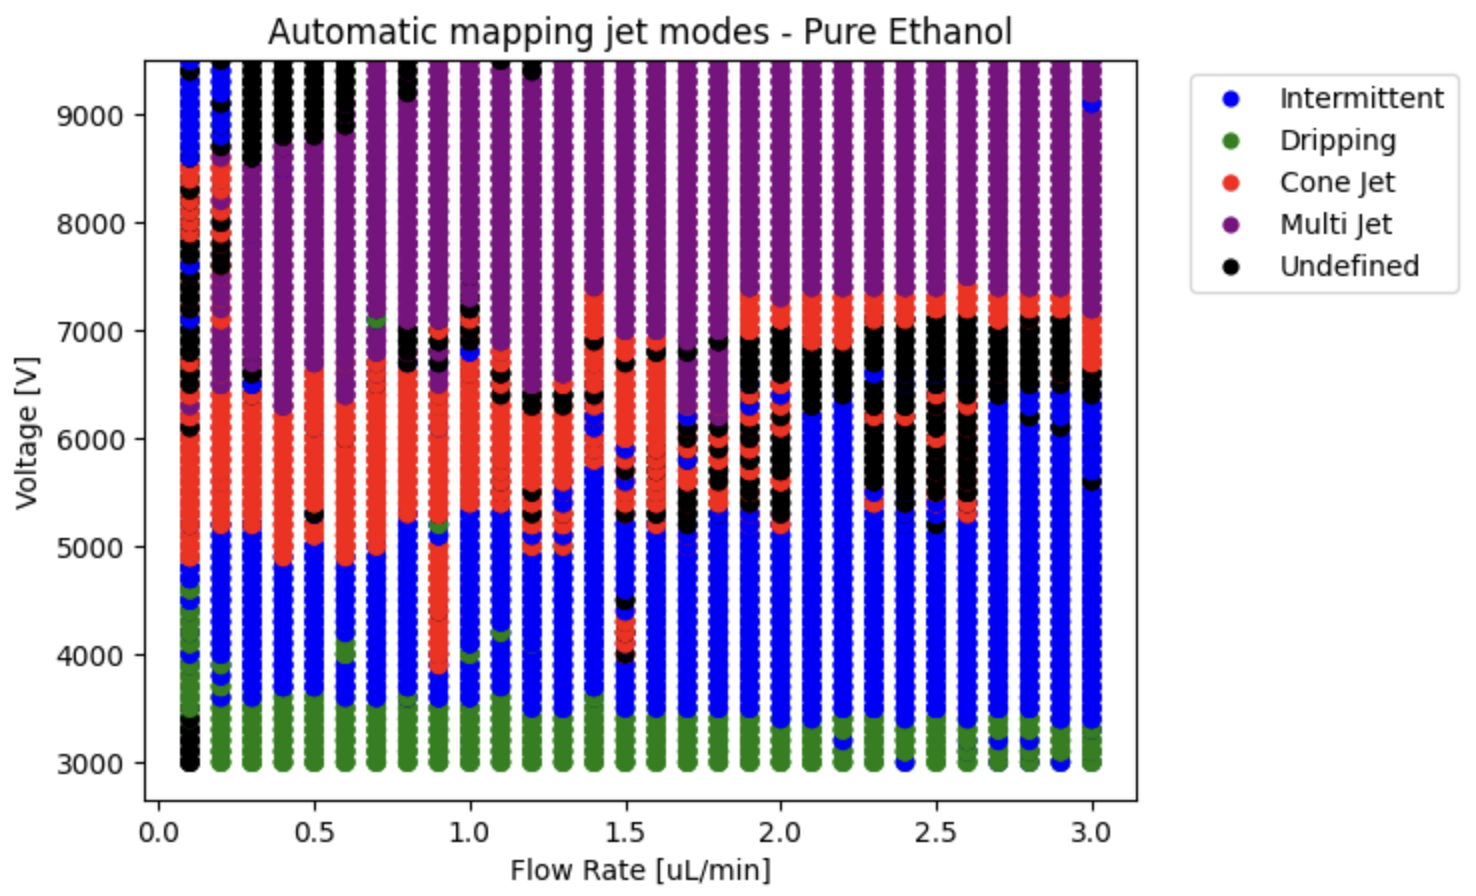
\includegraphics[width=15cm]{Figuras/report4/map-2023-03-02.png}
        \caption{Mapping Experiment for pure ethanol in ambient conditions. The map shows the stability region of each electrospraying mode in the voltage and flow rate range.}
        \label{fig:map3Data_fig}
    \end{figure}



\subsection{Control}

    The control sequence is the only from the list of sequences that actually uses the feedback classification value. 
    As it is a closed loop control, the controller must be able to stabilize the system in the desired conditions.
    A simple controller algorithm is represented in algorithm \ref{alg:simple_controller}, and it was used as a proof of concept.
    Its results can be seen in results section \ref{sec:controller_results}.

    \begin{algorithm}
        \caption{simple controller}\label{alg:simple_controller}
        \begin{algorithmic}
        \Function{controller}{$spray\_mode$} 
            
            \If{$spray\_mode$ = $'Intermittent'$ or $spray\_mode$ = $'Dripping'$}
                \State \Call{send\_voltage\_command}{$voltage$ + 100}
            \ElsIf{$spray\_mode$ = $'Multi Jet'$ or $spray\_mode$ = $'Corona'$}
                \State \Call{send\_voltage\_command}{$voltage$ - 100}
            \ElsIf{ $spray\_mode$ = $"Cone Jet"$}
                \Comment{Keep Stable}
            \EndIf

        \EndFunction
        \end{algorithmic}
    \end{algorithm}



\section{Chapter conclusion}

This chapter \ref{chap:Methodology} exhibits how the knowledge from chapter \ref{chap:lit_review} was implemented with a control and automation engineering approach in order to achieve the project goals. 
Next chapter \ref{chap:Results}, it will be discussed the results reached.




\clearpage